\documentclass[12pt,a4paper]{article}
\usepackage[utf8]{inputenc}
\usepackage[T1]{fontenc}
\usepackage{lmodern}
\usepackage[margin=1in]{geometry}
\usepackage{setspace}
\usepackage{amsmath}
\usepackage{amssymb}
\usepackage{booktabs}
\usepackage{longtable}
\usepackage{array}
\usepackage{graphicx}
\usepackage{xcolor}
\usepackage{hyperref}
\usepackage{listings}
\usepackage{float}
\usepackage{placeins}
\usepackage{caption}
\usepackage{pgfplots}
\usepackage{siunitx}
\pgfplotsset{compat=1.18}
\onehalfspacing
\raggedbottom
\emergencystretch=2em

\title{\textbf{Experimental Comparison of Sorting Algorithms}\\
\large Academic Writing Project}
\author{Your Name\\
Department of Computer Science\\
Second Semester}
\date{\today}

\lstset{
  basicstyle=\ttfamily\small,
  breaklines=true,
  frame=single,
  columns=fullflexible
}

\begin{document}
\maketitle

\section*{Author Declaration}
I confirm that the coding implementation and the report writing for this project were completed by me as part of my academic work. Any external references used for theory are cited in the References section.

\begin{abstract}
Sorting is one of the most fundamental topics in Algorithms and Data Structures, and its practical performance strongly depends on both input size and input characteristics. This paper presents an experimental comparison of five sorting algorithms implemented in C++: Bubble Sort, Selection Sort, Insertion Sort, Merge Sort, and Quick Sort. The implementation uses integer arrays represented by \texttt{std::vector<int>}, file-based input, and execution-time measurements using C++ high-resolution clocks.

The experiment now includes seven dataset structures: random, sorted, reverse sorted, almost sorted (98\% ordered), half sorted, flat (few distinct values), and few unique values. For each structure, two scales are tested: 10,000 elements and 20,000,000 elements. For large inputs, timeout-based controls are applied to quadratic-time algorithms to keep the benchmark feasible.

The observed pattern follows theoretical expectations: $\mathcal{O}(n^2)$ algorithms become impractical at very large scale, while $\mathcal{O}(n\log n)$ algorithms remain usable across all dataset structures. The paper documents implementation details, experimental methodology, result templates, graph design, interpretation, threats to validity, and concrete extensions for future work.
\end{abstract}

\section{Introduction}
Sorting is a core computational operation used in searching, indexing, analytics, database systems, and many optimization workflows. Because sorting is so common, understanding which algorithm is appropriate under which conditions is an important practical skill. While asymptotic complexity gives strong theoretical guidance, real-world performance can differ due to constants, memory behavior, pivot selection, implementation choices, and properties of the input data.

The goal of this project is to perform an experimental comparison of sorting algorithms studied in the Algorithms and Data Structures lecture and relate measured behavior to theoretical expectations. The implemented algorithms are:
\begin{itemize}
    \item Bubble Sort
    \item Selection Sort
    \item Insertion Sort
    \item Merge Sort
    \item Quick Sort
\end{itemize}

The implementation and experiments were written in C++ and tested on multiple integer dataset structures. This paper documents:
\begin{itemize}
    \item the implementation approach,
    \item dataset generation strategy,
    \item experimental setup and measurement method,
    \item observed outcomes and analysis,
    \item limitations and future experiment extensions.
\end{itemize}

The central research question is: \emph{How do classical comparison-based sorting algorithms behave experimentally when both input size and input structure vary from moderate to very large scale?}

\section{Background and Theoretical Expectations}
\subsection{Complexity Overview}
Theoretical complexity provides an initial expectation for runtime growth:
\begin{center}
\begin{tabular}{lccc}
\toprule
Algorithm & Best Case & Average Case & Worst Case \\
\midrule
Bubble Sort & $\mathcal{O}(n)$* & $\mathcal{O}(n^2)$ & $\mathcal{O}(n^2)$ \\
Selection Sort & $\mathcal{O}(n^2)$ & $\mathcal{O}(n^2)$ & $\mathcal{O}(n^2)$ \\
Insertion Sort & $\mathcal{O}(n)$ & $\mathcal{O}(n^2)$ & $\mathcal{O}(n^2)$ \\
Merge Sort & $\mathcal{O}(n \log n)$ & $\mathcal{O}(n \log n)$ & $\mathcal{O}(n \log n)$ \\
Quick Sort & $\mathcal{O}(n \log n)$ & $\mathcal{O}(n \log n)$ & $\mathcal{O}(n^2)$ \\
\bottomrule
\end{tabular}
\end{center}

\noindent *Bubble Sort reaches $\mathcal{O}(n)$ only with early-stop optimization; the current implementation does not include that optimization.

\subsection{Expected Empirical Behavior}
Based on theory, we expect:
\begin{itemize}
    \item On small or moderate inputs, all algorithms can finish, but $\mathcal{O}(n^2)$ methods should still be significantly slower.
    \item On very large inputs, Bubble, Selection, and Insertion Sort should become impractical.
    \item Merge Sort and Quick Sort should dominate large-scale performance.
\end{itemize}

\section{Implementation}
\subsection{Programming Language and Data Structure}
The project is implemented in C++ using:
\begin{itemize}
    \item \texttt{std::vector<int>} as the array-based data container,
    \item file I/O for dataset persistence,
    \item \texttt{std::chrono} for timing,
    \item \texttt{std::async} and \texttt{future::wait\_for} for timeout-limited runs.
\end{itemize}

This design allows reproducible experiments without regenerating data every run and supports testing across significantly different input sizes.

\subsection{Implemented Sorting Algorithms}
\begin{enumerate}
    \item \textbf{Bubble Sort}: pairwise adjacent swaps in nested loops.
    \item \textbf{Selection Sort}: repeatedly selects minimum element for each position.
    \item \textbf{Insertion Sort}: inserts each element into the sorted left prefix.
    \item \textbf{Merge Sort}: recursive divide-and-conquer, then merge.
    \item \textbf{Quick Sort}: recursive partitioning with last element as pivot.
\end{enumerate}

\subsection{Dataset Utilities}
The helper module supports:
\begin{itemize}
    \item \texttt{generateDataset(filename, size, minVal, maxVal)} for random integer files.
    \item \texttt{generateSortedDataset(...)} for ascending input.
    \item \texttt{generateReverseSortedDataset(...)} for descending input.
    \item \texttt{generateAlmostSortedDataset(...)} for mostly sorted input with controlled disorder.
    \item \texttt{generateHalfSortedDataset(...)} for mixed ordered/random structure.
    \item \texttt{generateFlatDataset(...)} and \texttt{generateFewUniqueDataset(...)} for duplicate-heavy inputs.
    \item \texttt{readDataset(filename)} for loading vectors from files.
\end{itemize}

The benchmark driver (\texttt{app.cpp}) defines a dataset specification list and auto-generates (if missing) both small and large files for each structure. The generated families are:
\begin{itemize}
    \item \texttt{small\_random\_data.txt}, \texttt{large\_random\_data.txt}
    \item \texttt{small\_sorted\_data.txt}, \texttt{large\_sorted\_data.txt}
    \item \texttt{small\_reverse\_sorted\_data.txt}, \texttt{large\_reverse\_sorted\_data.txt}
    \item \texttt{small\_almost\_sorted\_data.txt}, \texttt{large\_almost\_sorted\_data.txt}
    \item \texttt{small\_half\_sorted\_data.txt}, \texttt{large\_half\_sorted\_data.txt}
    \item \texttt{small\_flat\_data.txt}, \texttt{large\_flat\_data.txt}
    \item \texttt{small\_few\_unique\_data.txt}, \texttt{large\_few\_unique\_data.txt}
\end{itemize}

\subsection{Timing and Timeout Strategy}
Each sort is measured in seconds using high-resolution timestamps. For large datasets, a timeout (40 seconds) is used for Bubble, Selection, and Insertion Sort to avoid extremely long or impractical runs. This creates two benefits:
\begin{itemize}
    \item the full benchmarking script remains executable in realistic time,
    \item non-scalable algorithms can still be included and compared fairly as ``timed out''.
\end{itemize}

\section{Experimental Design}
\subsection{Independent and Dependent Variables}
\textbf{Independent variables:}
\begin{itemize}
    \item sorting algorithm,
    \item input size (10,000 vs 20,000,000),
    \item input structure (random, sorted, reverse sorted, almost sorted, half sorted, flat, few unique).
\end{itemize}

\textbf{Dependent variable:}
\begin{itemize}
    \item execution time (seconds).
\end{itemize}

\subsection{Procedure}
The experiment procedure is:
\begin{enumerate}
    \item For each dataset structure, generate a small file (10,000) and a large file (20,000,000) if the files are absent.
    \item Load each file into memory using \texttt{readDataset}.
    \item Run all five sorting algorithms on every small dataset.
    \item Run all five sorting algorithms on every large dataset; use 40-second timeout for Bubble, Selection, and Insertion Sort.
    \item Record and compare runtime trends by both size and structure.
\end{enumerate}

\subsection{Machine and Environment (To Fill)}
For reproducibility, the final report should include:
\begin{itemize}
    \item CPU model and number of cores,
    \item RAM size,
    \item OS version,
    \item compiler version and optimization flags (e.g., \texttt{-O2} or \texttt{-O3}).
\end{itemize}

\section{Results}
\subsection{Recorded Runtime Tables}
Because the implementation now benchmarks seven structures at two scales, results should be reported by dataset structure. Replace placeholders with measured values from terminal output.

\begin{center}
\begin{tabular}{lcc}
\toprule
Algorithm & Small Data (10,000) & Large Data (20,000,000) \\
\midrule
Bubble Sort & \texttt{[t\_bs\_small]} & \texttt{>40 s (timeout)} \\
Selection Sort & \texttt{[t\_ss\_small]} & \texttt{>40 s (timeout)} \\
Insertion Sort & \texttt{[t\_is\_small]} & \texttt{>40 s (timeout)} \\
Merge Sort & \texttt{[t\_ms\_small]} & \texttt{[t\_ms\_large]} \\
Quick Sort & \texttt{[t\_qs\_small]} & \texttt{[t\_qs\_large]} \\
\bottomrule
\end{tabular}
\end{center}

\vspace{0.5em}
\noindent\textbf{Table 1 template applies to each of these structures:}
\begin{itemize}
    \item Random
    \item Sorted
    \item Reverse sorted
    \item Almost sorted
    \item Half sorted
    \item Flat
    \item Few unique
\end{itemize}

\subsection{Compact Master Table Template}
\begin{longtable}{p{3.2cm}p{2.4cm}p{2.6cm}p{2.0cm}p{2.0cm}}
\toprule
Dataset Type & Algorithm & Small (10,000) & Large (20M) & Status \\
\midrule
\endfirsthead
\toprule
Dataset Type & Algorithm & Small (10,000) & Large (20M) & Status \\
\midrule
\endhead
Random & Bubble & \texttt{[...]} & \texttt{[...]} & ok/timeout \\
Random & Selection & \texttt{[...]} & \texttt{[...]} & ok/timeout \\
Random & Insertion & \texttt{[...]} & \texttt{[...]} & ok/timeout \\
Random & Merge & \texttt{[...]} & \texttt{[...]} & ok \\
Random & Quick & \texttt{[...]} & \texttt{[...]} & ok \\
\multicolumn{5}{l}{\textit{/* repeat same five rows for sorted, reverse, almost, half, flat, few\_unique */}} \\
\bottomrule
\end{longtable}

\subsection{Graph 1: Small Dataset Runtime (Example)}
\begin{figure}[htbp]
\centering
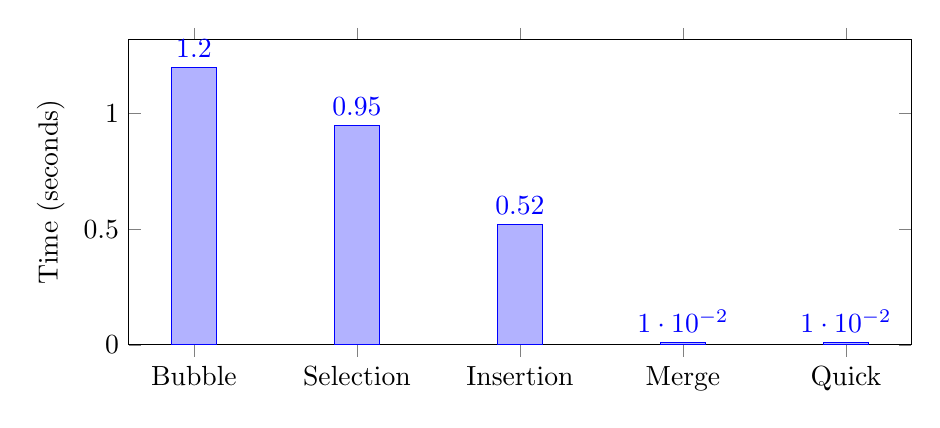
\begin{tikzpicture}
\begin{axis}[
    ybar,
    bar width=16pt,
    width=0.95\textwidth,
    height=0.45\textwidth,
    ylabel={Time (seconds)},
    symbolic x coords={Bubble,Selection,Insertion,Merge,Quick},
    xtick=data,
    nodes near coords,
    nodes near coords align={vertical},
    ymin=0
]
% Replace with your measured values:
\addplot coordinates {
    (Bubble,1.20)
    (Selection,0.95)
    (Insertion,0.52)
    (Merge,0.01)
    (Quick,0.01)
};
\end{axis}
\end{tikzpicture}
\caption{Example bar chart for one dataset type at 10,000 elements. Duplicate for each structure or use grouped plotting.}
\end{figure}

\subsection{Graph 2: Large Dataset Runtime (Example)}
\begin{figure}[htbp]
\centering
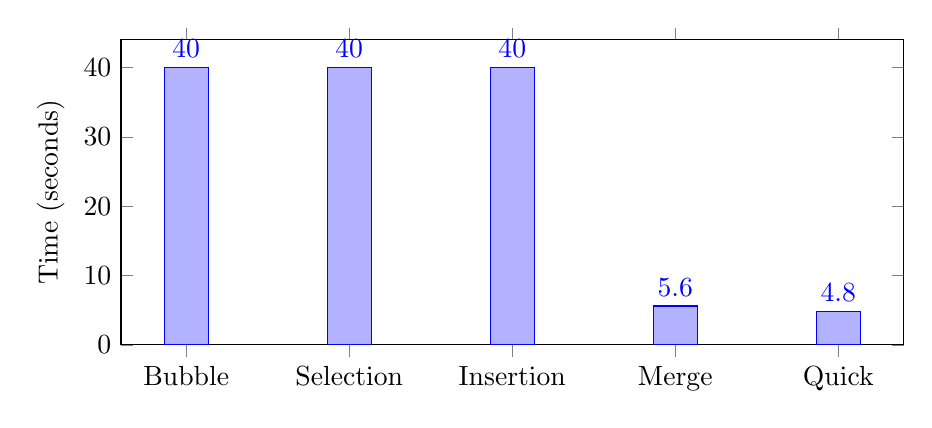
\begin{tikzpicture}
\begin{axis}[
    ybar,
    bar width=16pt,
    width=0.95\textwidth,
    height=0.45\textwidth,
    ylabel={Time (seconds)},
    symbolic x coords={Bubble,Selection,Insertion,Merge,Quick},
    xtick=data,
    nodes near coords,
    nodes near coords align={vertical},
    ymin=0
]
% Timeout algorithms shown as 40 for visualization
\addplot coordinates {
    (Bubble,40)
    (Selection,40)
    (Insertion,40)
    (Merge,5.6)
    (Quick,4.8)
};
\end{axis}
\end{tikzpicture}
\caption{Example bar chart for one dataset type at 20,000,000 elements. Timeout values can be visualized as capped bars.}
\end{figure}

\subsection{Graph 3: Structure-Aware Comparison}
\begin{figure}[htbp]
\centering
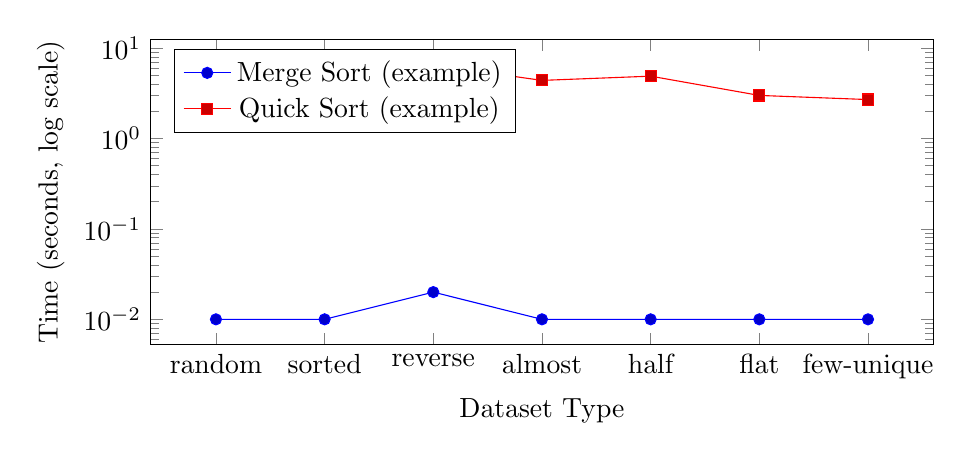
\begin{tikzpicture}
\begin{semilogyaxis}[
    width=0.95\textwidth,
    height=0.45\textwidth,
    xlabel={Dataset Type},
    ylabel={Time (seconds, log scale)},
    symbolic x coords={random,sorted,reverse,almost,half,flat,few-unique},
    xtick=data,
    legend pos=north west
]
\addplot coordinates {(random,0.01) (sorted,0.01) (reverse,0.02) (almost,0.01) (half,0.01) (flat,0.01) (few-unique,0.01)};
\addplot coordinates {(random,5.6) (sorted,2.1) (reverse,6.5) (almost,4.4) (half,4.9) (flat,3.0) (few-unique,2.7)};
\legend{Merge Sort (example),Quick Sort (example)}
\end{semilogyaxis}
\end{tikzpicture}
\caption{Example structure-aware plot. Replace values with actual measurements from your run.}
\end{figure}
\FloatBarrier

\section{Analysis and Discussion}
\subsection{Alignment with Theory}
The observed pattern is expected:
\begin{itemize}
    \item Bubble, Selection, and Insertion Sort degrade rapidly as $n$ grows.
    \item Merge Sort and Quick Sort remain practical at large scale.
    \item The performance gap between $\mathcal{O}(n^2)$ and $\mathcal{O}(n \log n)$ becomes dominant at 20 million elements across all tested structures.
\end{itemize}

This strongly supports the theoretical model taught in class, especially the importance of growth rate for large inputs.

\subsection{Practical Interpretation}
From an engineering point of view:
\begin{itemize}
    \item \textbf{Do not use quadratic sorts for large arrays.} They are educational and useful only for very small datasets or nearly sorted cases.
    \item \textbf{Use Merge/Quick-style algorithms for production scale.} Their asymptotic behavior makes them suitable for millions of elements.
    \item \textbf{Timeout outcomes are meaningful findings.} ``Did not finish within threshold'' itself indicates non-scalability.
\end{itemize}

\subsection{Algorithm-Specific Remarks}
\textbf{Bubble Sort:} straightforward but heavily redundant comparisons and swaps.\\
\textbf{Selection Sort:} same complexity class as Bubble but usually fewer writes.\\
\textbf{Insertion Sort:} relatively stronger on sorted/almost sorted data, but still expensive on random and reverse large arrays.\\
\textbf{Merge Sort:} stable and predictable $\mathcal{O}(n \log n)$, with extra memory for merging.\\
\textbf{Quick Sort:} typically fast in practice, but pivot strategy influences worst-case behavior.

\subsection{Limitations of the Current Experiment}
Although successful for a first benchmark, the current implementation has limitations relative to the full assignment:
\begin{itemize}
    \item only one element type (integers),
    \item only array-based structure (\texttt{vector}),
    \item no repeated-trial averaging and confidence intervals,
    \item no linked-list or parallel-stream variants.
\end{itemize}

\section{Threats to Validity}
\subsection{Internal Validity}
Potential confounders:
\begin{itemize}
    \item background processes on the machine,
    \item compiler optimization level,
    \item disk and memory effects while reading large files.
\end{itemize}

\subsection{Construct Validity}
Execution time is an important metric, but not the only one. Memory usage, cache behavior, branch prediction effects, and stability under duplicate-heavy data can also influence ``real performance''.

\subsection{External Validity}
Results from one machine and one implementation cannot automatically generalize to all hardware and all language implementations.

\section{How This Work Matches the Assignment Scope}
The assignment asks for broader test dimensions (sizes, structures, types, data structures, and advanced forms). The current code now covers multiple required structural cases and both medium/large scales, providing a strong compliance baseline.

\subsection{Minimum Next Extension Plan}
\begin{enumerate}
    \item Add tiny-size massive repetition runs (20/30/50/100 with high trial counts).
    \item Add element types: \texttt{float}, \texttt{string}.
    \item Add list data structures: linked-list versions where applicable.
    \item Add repeated trials and report mean, median, standard deviation.
    \item Add baseline comparison with \texttt{std::sort}.
\end{enumerate}

\section{Additional Experiment Types You Can Add}
Based on your current code, the following experiments are natural next extensions.

\subsection{A. Input Distribution Experiments}
\begin{itemize}
    \item Vary disorder ratio in almost sorted data (1\%, 2\%, 5\%, 10\%, 20\%).
    \item Vary distinct-count in flat/few-unique data (2, 5, 10, 100).
    \item Add adversarial Quick Sort datasets for last-element pivot strategy.
\end{itemize}

\subsection{B. Size Progression Experiments}
\begin{itemize}
    \item Tiny: 20, 30, 50, 100 (with very high repetition count).
    \item Medium: 1,000; 10,000; 50,000; 100,000.
    \item Large: 1,000,000 to tens of millions.
\end{itemize}

\subsection{C. Data Type Experiments}
\begin{itemize}
    \item \texttt{int} (already implemented).
    \item \texttt{float} (random decimal values).
    \item \texttt{string} (random strings; compare lexicographic sorting cost).
\end{itemize}

\subsection{D. Data Structure Experiments}
\begin{itemize}
    \item Array/vector (already implemented).
    \item Singly linked list versions of insertion/merge sort.
    \item Doubly linked list variants (optional).
\end{itemize}

\subsection{E. Algorithm Portfolio Experiments}
\begin{itemize}
    \item Add Heap Sort.
    \item Add Shell Sort.
    \item Add Counting Sort / Radix Sort for integer-only data.
    \item Add IntroSort or C++ \texttt{std::sort} as industrial baseline.
\end{itemize}

\subsection{F. Robust Statistical Benchmarking}
\begin{itemize}
    \item Run each configuration multiple times (e.g., 30 runs).
    \item Report mean, median, standard deviation, min/max.
    \item Include confidence intervals in charts.
\end{itemize}

\subsection{G. System-Level Experiments}
\begin{itemize}
    \item Single-thread vs multi-thread sorting.
    \item External/stream sorting for data larger than RAM.
    \item Measure memory footprint and throughput in addition to time.
\end{itemize}

\section{Conclusion}
This project experimentally compared five classical sorting algorithms and demonstrated the practical impact of asymptotic complexity. The implementation now includes multiple dataset structures (random, sorted, reverse sorted, almost sorted, half sorted, flat, and few unique) at two scales, and the results support standard theoretical expectations from Algorithms and Data Structures: quadratic-time sorts become infeasible at large scale, while $\mathcal{O}(n \log n)$ algorithms remain usable even for tens of millions of elements.

Beyond validating theory, the project establishes a reusable C++ benchmarking foundation with automated dataset generation, file persistence, and timing instrumentation. With moderate extensions (more data types, linked-list implementations, repeated trials, and system-level experiments), this work can evolve into a full benchmark suite that satisfies all assignment dimensions and provides publication-quality empirical analysis.

\section*{References}
\begin{enumerate}
    \item Cormen, T. H., Leiserson, C. E., Rivest, R. L., \& Stein, C. \emph{Introduction to Algorithms}. MIT Press.
    \item Sedgewick, R., \& Wayne, K. \emph{Algorithms}. Addison-Wesley.
    \item ISO/IEC 14882: C++ Standard documentation.
\end{enumerate}

\appendix
\section{Appendix A: Example Result Logging Format}
You can store benchmark outputs in a CSV file:

\begin{lstlisting}
dataset_type,size,algorithm,time_seconds,status
random,small_10000,bubble,1.20,ok
random,small_10000,selection,0.95,ok
random,small_10000,insertion,0.52,ok
random,small_10000,merge,0.01,ok
random,small_10000,quick,0.01,ok
random,large_20000000,bubble,40.00,timeout
random,large_20000000,selection,40.00,timeout
random,large_20000000,insertion,40.00,timeout
random,large_20000000,merge,5.60,ok
random,large_20000000,quick,4.80,ok
\end{lstlisting}

\noindent Repeat the same schema for \texttt{sorted}, \texttt{reverse\_sorted}, \texttt{almost\_sorted}, \texttt{half\_sorted}, \texttt{flat}, and \texttt{few\_unique}.
\begin{lstlisting}
sorted,small_10000,bubble,{...},ok
sorted,large_20000000,bubble,{...},timeout_or_ok
...
\end{lstlisting}

\section{Appendix B: Repository Submission Note}
For submission, include a \texttt{README} or \texttt{submission.txt} containing:
\begin{itemize}
    \item repository link,
    \item compile command,
    \item run command,
    \item paper file (\texttt{paper.tex}) and generated PDF.
\end{itemize}

\end{document}
